\documentclass[11pt]{article}
\usepackage[a4paper,width=150mm,top=25mm,bottom=25mm,bindingoffset=6mm]{geometry}
\usepackage{fancyhdr}
\pagestyle{fancy}
\usepackage[final]{graphicx}
\usepackage{subcaption}



%Gummi|065|=)
\title{\textbf{Virtual Parking System}}
\author{Luca Accorsi}
\date{}
\begin{document}

\maketitle

\section{Overview}
This application should be a working prototype of a system that aims to manage a smart virtual parking area. The system is virtual in the sense that the components (sensors, cars, etc) are not real but are software components that simulate a plausible behavior. The substitution of simulated components with real devices should be straightforward.

\section{Requirements}
It is required the development of a smart parking system to handle approximately some hundreds of parking places. A park is a $n$ x $m$ matrix where each cell could be a parking place or a street block. The park designers will take care to design a drivable park, that is a park where drivers are able to correctly move. Each parking place contains a parking sensor able to acquire information about the presence or absence of a car. The sensor is handled by a simple computer equipped with a network interface that could be used to work with networks. Each sensor has also the possibility to create a very small, one-cell broad, local network area that could be useful to communicate with neighbors (other sensors or clients). The system should give drivers the possibility to quickly identify a free near parking place and to locate a previously parked car. It is thus required a client application. To avoid services disruption in case the server doesn't properly work, it is required that the system is able to work in both a centralized way but it should also be able to perform some basic functionalities in a fully distributed way.

\section{Requirements analysis}
From the requirements analysis can be stated that the main entities that compose the system are:
\begin{itemize}
\item an \textbf{environment}: it is where the parking area is placed and everything takes place. It is a grid-based area, that is an ($n$ x $m$) matrix where each cell could be a street block or a parking place.
\item a \textbf{sensors layer}: each car parking place is equipped with a parking sensor, a computing processor and a network interface.
\item a \textbf{server application}: since the system should work in a centralized way, a central server (or many of them) is (are) required.
\item some \textbf{client applications}: that is, applications that drivers will use to identify a free near parking place or to locate a previously parked car.
\end{itemize}
The main functions that the system has to accomplish could be summarized with:
\begin{itemize}
\item providing parking support;
\item provide some basic information when the server is not available.
\end{itemize}

The system should face the following complexity aspects:
\begin{itemize}
\item it is composed by a dynamic and possibly large set of components. At any given moment the number of clients is unpredictable.
\item it is open, that is, components (clients but also sensors) could be added or removed while the system is working.
\item it is heterogeneous, clients, server and sensors application may be written in different programming languages.
\item it should work in a centralized and decentralized/distributed way.
\item the interactions are asynchronous and loose coupled.
\item the components are situated in a (virtual) world.
\item there may be component failures.
\end{itemize}

\section{Problem analysis}
The problem analysis could start from a very high level view. From the requirements could be stated that the whole system, from the \textbf{structure} point of view, is composed by the following sub-systems:
\begin{itemize}
\item the sensors spread across the park
\item the clients
\item a server
\end{itemize}
The whole system expected \textbf{behavior} is thoroughly explained in the requirements section but the behavior of each sub-system will be deeply analyzed in the following sub-sections. The \textbf{interactions} that occurs in the system may be initially introduced in a simplified version by the Figure 1.
\begin{figure}
  \centering
	\includegraphics[scale=1]{system}
  \caption{High level system view}
\end{figure}
Here it could be seen that two different kind of possible interactions exist: global (\textbf{g}) and local (\textbf{l}) ones. For global interaction it is meant an interaction that exploit a centralization element reachable independently from the distance from its physical location, the server in this case, while a local interaction is an interaction that could happen in a well defined and typically small area, for eg. sensor-sensor or client-sensor communications.
In the following subsections there will be a more focused analysis of each sub-system.
\subsection{Sensor model}
Each parking place is provided of a parking sensor, from now it will be called just sensor, able to perform the above described functionalities. The sensor is a simple proactive entity composed by two parts: a sensing unit and a control unit. The sensing unit is the software component that drives the physical (or virtual) input device (for eg. a proximity or obstacle physical sensor) while the control unit is the component where the application logic resides and that controls the sensing unit. The behavior of the sensor could be discussed on two different levels. According to the customer requirements it is necessary that the system is able to work in both a centralized and a distributed way, this is reflected in the two different and integrated behaviors that the sensor performs: a server-oriented and a neighbor-oriented one. The server-oriented behavior could be described by an infinite loop where sense, process and act operations are continuously performed. In particular the sense operation retrieves data from the sensing unit, the process operation adapts, changes, translates the data in some kind of information (for eg. a JSON message) and the act operation uses some actuator to produce an effect (for eg. message sending using the network interface). An informal picture could be seen in Figure 2.
\begin{figure}
  \centering
	\includegraphics[scale=1]{sensor_server_oriented_behavior}
  \caption{Server-oriented sensor behavior}
\end{figure}
In the neighbor-oriented behavior, the sensor should be able receive requests from clients, check if it is able to satisfy them and if not, spread the request to neighbor sensors. An informal picture could be seen in Figure 3.
\begin{figure}
  \centering
	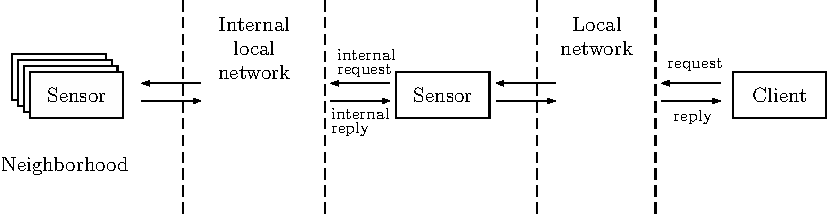
\includegraphics[scale=1]{sensor_neighbor_oriented_behavior}
  \caption{Neighbor-oriented sensor behavior}
\end{figure}
\subsection{Server model}
The server is a centralization element and a complex proactive and reactive entity, it receives state messages from the sensors and requests from clients. The server can build a complete view of the park since it receives information from all the sensors, and update this knowledge when necessary. The server could be seen in a simplified way as composed by a sensors-handler module and a client-handler module. The sensors-handler module receives messages from sensors and updates the internal server state while the clients-handler receives messages from clients. A client message is essentially a one-time welcome request where the client asks the server for an updated version of the world. After the first request the client will never contact the server again. The server will publish new updated world versions each time the sensor-handler finds out that the server internal state is different from the partial world description received from a sensor message. An informal picture could be seen in Figure 4.
\begin{figure}
  \centering
	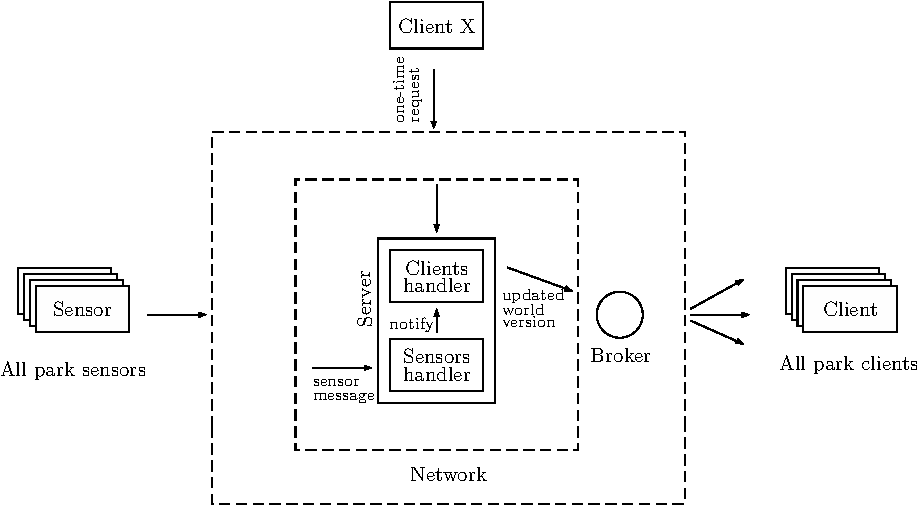
\includegraphics[scale=1]{server}
  \caption{Server behavior and interaction}
\end{figure}

\subsection{Client model}
Each driver is provided of an application that should grant him some smart parking support. The application should help to find out a near free place and to locate a previously parked car. The client application, from now on just client, is a \emph{thick} client composed by a user-interaction module, a server-interaction module and an emergency neighbor-interaction module. The user interaction-module should handle the user actions, that is: park a car, remove a parked one, locate a previously parked car and find the nearest free parking place. The server-interaction module should contact the server for the one-time welcome handshake and update the internal client knowledge each time the server publishes a new world version. Finally, the neighbor-interaction module should provide support in local interactions with near sensors when the server is not available. An informal picture could be seen in Figure 5.
\begin{figure}
  \centering
	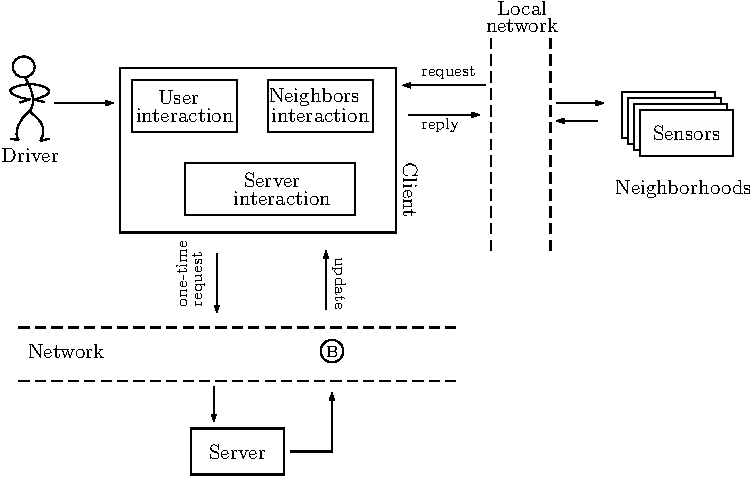
\includegraphics[scale=1]{client}
  \caption{Client behavior and interaction}
\end{figure}

\subsection{Complexity remarks}
The system is an ensemble of different standalone applications, then it raises all the problematics of distributed systems and applications integration. First of all it is absolutely necessary that the applications will be designed with the aim of minimizing the dependencies between them. This is a key aspects in developing an integrated application system because if the sub-systems are not loose coupled a small change in one could cause a complete and expensive system refactoring. One of the most important things to decide is how to carry on the integration between the different applications (or sub-systems). Since loose coupling is required a natural integration approach that could be used is communication via messaging that aims at minimizing the assumptions between components. Message passing communication raises other problems: the selection of a standard data format, the decision between direct or indirect (channel) communication and a more complex programming model where asynchronous and callback styles rule. Another important aspect concerns components failures and the possibility to replace sub-systems without stopping the whole system. All these aspects will be considered during the design and development of the different subsystems and in Section 5.5 there will be a summary of the most important strategies adopted to faces them.

\section{System Design}
In this section is described the system design using some formal UML diagrams.

\subsection{Sensor design}
The UML diagrams in Figure 6 describe the structure dimension of a sensor. The main elements are:
\begin{figure}
  \centering
	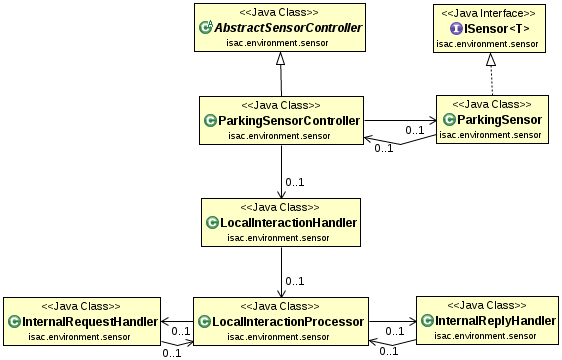
\includegraphics[scale=0.8]{sensorUML}
  \caption{Sensor UML structure diagram}
\end{figure}
\begin{itemize}
\item \emph{ISensor}: it defines the interface of a generic sensor in terms of available operations.
\item \emph{ParkingSensor}: it implements \emph{ISensor} as a simple virtual parking sensor able to sense a virtual environment to check if there is a car in the parking place where it is placed or not. It is the sensing unit described in Section 4.1.
\item \emph{AbstractSensorController}: it is an abstract class that defines the structure of the behavior of a general sensor controller unit, it could be thought as the abstract model of the control unit described in Section 4.1 while \emph{ParkingSensorController} is the concrete one. It defines the sensor behavior in terms of an infinite loop of sense, process and act (abstract) operations.
\item \emph{ParkingSensorController}: it is where the operations described in \emph{AbstractSensorController} are concretely defined. It also provide the support for the local interaction with clients and other sensors and the sensor-to-server communication.
\item \emph{LocalInteractionHandler}: it is the daemon that receives and sends local messages from and to clients when the server is not available. It is implemented using an \emph{event loop} structure so as to process one message at a time to avoid concurrency troubles. Once a client request (\emph{LocalRequest}) is received it is forwarded to the \emph{LocalInteractionProcessor} that is the component that has the knowledge to decide what to do. A client could interact (send and receive messages) with sensors that are at most one-block distant.
\item \emph{LocalInteractionProcessor}: it is the component able to process all the different possible local messages: client-to-sensor messages (\emph{LocalRequest}), sensor-to-client messages (\emph{LocalReply}) and sensor-to-sensor messages (\emph{InternalRequest} and \emph{InternalReply}). Once a message of one of the previous type is received the \emph{LocalInteractionProcessor} checks if this sensor is able to satisfy the request or not (for eg. if the sensor is free or contains the searched car). If it is, one of the following actions is performed:
\begin{itemize}
\item \emph{LocalRequest}: direct interaction through a newly built \emph{LocalReply} message with the client that required something.
\item \emph{LocalReply}: this message can't be received from sensors.
\item \emph{InternalRequest}: an \emph{InternalReply} is created and spread to neighbors sensors.
\item \emph{InternalReply}: if this sensor is the one directly contacted by the client a \emph{LocalReply} is created and sent to the client otherwise the \emph{InternalReply} is spread to neighbors sensors. The \emph{LocalInteractionProcessor} also takes care to avoid endless messages circulation between neighbor sensors. Two sensors are considered neighbors if their block distance is at most one. The \emph{LocalReply} is always sent to the client from the sensor first contacted from the client, this behavior follows the strong assumption that the client has not moved while the sensors are processing the request, assumption that in real scenarios is hardly ever true.
\end{itemize}
If not the message is spread to all the neighbors sensors.
\item \emph{InternalRequestHandler}: daemon implemented using an event loop structure that manages, that is sends and receives, \emph{InternalRequest}(s). Once a request is received, it is forwarded to the \emph{LocalInteractionProcessor}.
\item \emph{InternalReplyHandler}: it is the \emph{InternalRequestHandler} dual component. It obviously handles \emph{InternalReply}(s).
\end{itemize}

\subsection{Client design}
The UML diagrams in Figure 7 describe the structure dimension of a client. The main elements are:
\begin{figure}
  \centering
	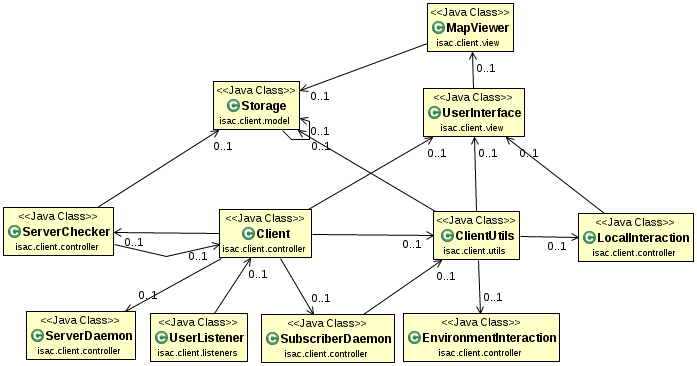
\includegraphics[scale=0.65]{clientUML}
  \caption{Client UML structure diagram}
\end{figure}
\begin{itemize}
\item \emph{Client}: it is the application entry point where most of the services are started.
\item \emph{ServerDaemon}: it receives \emph{pings} from the server when the latter is correctly working and updates a variables that maintains the last reception time. The server will send new world information only when changes happen. If the server does not send this information within a prefixed amount of time from the last reception, the \emph{ServerChecker} sets a \emph{serverOffline} variable as \emph{true}. When \emph{serverOffline} is \emph{true} the client will use local interactions with sensors instead of server information. It also performs the initial one-time client request, otherwise the server won't send updated world information till a changes occur.
\item \emph{ServerChecker}: it periodically checks the amount of time between the last receipt server ping and the current time. If this value is greater than a prefixed threshold it sets the \emph{serverOffline} variable as \emph{true}.
\item \emph{SubscriberDaemon}: it receives raw world information (a map of sensor names to sensor states) from the server and build the internal client world representation as a graph of sensor and street nodes that will be used to perform the required functionalities (eg. free parking place search using a breadth-first search and car location computing the shortest-path from single source using the Dijkstra algorithm).
\item \emph{Storage}: it is where all the client knowledge is stored, it is implemented using the Singleton pattern for convenience.
\item \emph{ClientUtils}: it is where are implemented the client required functionalities (park, remove car, movements, ...). It supports functionalities when the whole park knowledge is available, that is when the server is correctly working, but also when just local interactions are possible.
\item \emph{LocalInteraction}: it sends and receives messages to and from sensors when the server is not available. Once a message is receives it updates the user interface to show information to the user.
\item \emph{EnvironmentInteraction}: since the environment is virtual, this class provides functionalities to interact (via messages) with the environment (for eg. to let know a sensor that a driver has decided to park in the parking place that the first is checking).
\item \emph{UserListener}: it is the bridge between the user and the application.
\item \emph{UserInterface}: it is the client simple user interface.
\item \emph{MapViewer}: it is a panel that displays the map when complete information are available otherwise few textual information when local interactions need to be carried on.
\end{itemize}

\subsection{Server design}
The UML diagrams in Figure 8 describe the structure dimension of the server application. The main elements are:
\begin{figure}
  \centering
	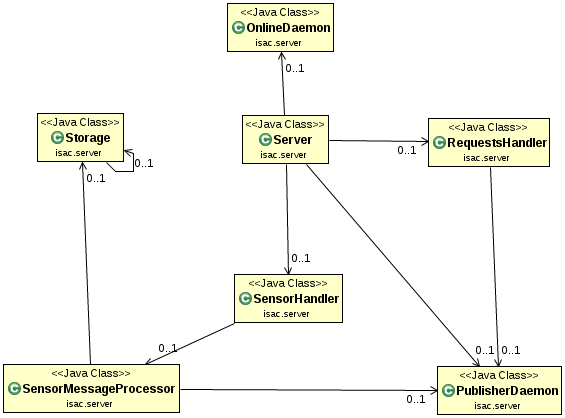
\includegraphics[scale=0.8]{serverUML}
  \caption{Server UML structure diagram}
\end{figure}
\begin{itemize}
\item \emph{Server}: it is the server entry point where most of the services are started.
\item \emph{OnlineDaemon}: it periodically sends pings to all available clients to let them know that the server is correctly working.
\item \emph{SensorHandler}: it receives messages from all the sensors. Each sensor message is processed by the \emph{SensorMessageProcessor}.
\item \emph{SensorMessageProcessor}: it processes sensor messages, that is it translate individual raw data into aggregate information. It is implemented following the event loop structure in order to avoid concurrency trouble in managing many messages each second.
\item \emph{Storage}: it is where the server stores its knowledge.
\item \emph{RequestsHandler}: it receives the one-time client request when a new client requires updated world information, that is when the client starts. Once a request arrives, the \emph{RequestsHandler} notifies the \emph{PublisherDaemon} to send the updated world version to every available clients.
\item \emph{PublisherDaemon}: it sends updated world information when required, that is when something has changed or when someone required it.
\end{itemize}
\subsection{Environment design}
The system lives in a virtual world, the environment should represent this world. The UML diagrams in Figure 9 describe the structure dimension of the environment. The main elements are:
\begin{figure}
  \centering
	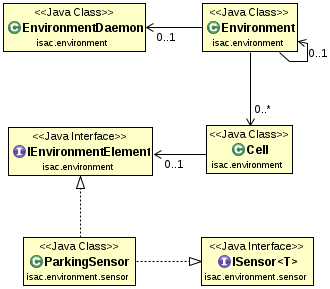
\includegraphics[scale=0.8]{environmentUML}
  \caption{Environment UML structure diagram}
\end{figure}
\begin{itemize}
\item \emph{Environment}: it represents the virtual world as an $n$ x $m$ matrix of \emph{Cell}(s) that may or not contain sensors. Each sensor checks the environment to understand if there is a car in front of him or not.
\item \emph{Cell}: it represents a single environment element. 
\item \emph{IEnvironmentElement}: it is an interface that defines that all environment elements must have a position.
\item emph{EnvironmentDaemon}: it receives messages from clients and updates the environment state.
\end{itemize}
The environment could be easily defined from a textual file using the \emph{Configurator} class (not displayed in the above UML diagram). The environment software layer provides also a simple command line interpreter that could be used to replace broken sensors.

\subsection{Facing complexity aspects}
A message oriented middleware MOM (RabbitMQ) has been adopted to solve the application integration problems, it provides space-temporal-referential decoupling thanks to the channel abstraction. Each sub-system knows which channel will be used and for which purpose. The messages has been defined in JSON that is a standard format for defining the syntax of a message, this way applications interoperability should be granted independently from the programming language adopted. One of the drawbacks of message oriented programming consists in the definition of callbacks to handle messages reception. To avoid concurrency problems when it was necessary to update shared data structures an event loop structure has been adopted to handle one message at a time in a FIFO fashion. The local interactions between sensors give rise to the emergent properties of searching for a position in a distributed system. Components may fail, if a sensor broke the system allows to easily replace it without stopping the whole system. Also the server may fail, if it happens clients could use local interactions with sensor until a new server instance is online. A broken server could be replace with a working one in every moment without having to reboot the whole system. This is possible thanks the indirection layer provided by channels of the MOM.

\end{document}
